% % % % % % % % % % % % % % % % % % % % % 
% results.tex - Ian Huston
% $Id: results.tex,v 1.34 2009/11/30 12:11:02 ith Exp $
% % % % % % % % % % % % % % % % % % % % % 
% Redefine CVSRevision for this section
\renewcommand{\CVSrevision}{\version$Id: results.tex,v 1.34 2009/11/30 12:11:02 ith Exp $}

% % % % % % % % % % % % % % % % % % % % % % % % % % % % % % % % 
% =========================================================== %
% % % % % % % % % % % % % % % % % % % % % % % % % % % % % % % %
\chapter{Results and Future Work}
\label{ch:results}
% % % % % % % % % % % % % % % % % % % % % % % % % % % % % % % % 
% =========================================================== %
% % % % % % % % % % % % % % % % % % % % % % % % % % % % % % % %


% % % % % % % % % % % % % % % % % % % % % % % % % % % % % % % % 
% =========================================================== %
% % % % % % % % % % % % % % % % % % % % % % % % % % % % % % % %
\section{Introduction}
\label{sec:intro-res}
% % % % % % % % % % % % % % % % % % % % % % % % % % % % % % % % 
% =========================================================== %
% % % % % % % % % % % % % % % % % % % % % % % % % % % % % % % %

The main result of Part~\ref{part:numerical} of this thesis is the numerical
integration of
the Klein-Gordon equation of motion for second order scalar field
perturbations, \eq{eq:KG2-fourier-sr-num}. The slow
roll approximation of the source term for second order perturbations was employed,
but the complete versions of the evolution equations were used for the
background and first
order perturbations. In this chapter the results of the numerical calculation will be
presented. This represents the
first step towards a full calculation of the Klein-Gordon equation at second order.
In addition to the new results obtained, plans will be described for future
work aimed at improving the numerical system and increasing its range
of applicability. 

As a proof of concept, the numerical system was tested with four different
potentials, $V(\vp)=\msqphisq$, $\lambdaphifour$, $\phitwooverthree$ and
$\msqphisqwithV$, and results computed across three
different $k$ ranges. As expected, the second order perturbation for a single,
slowly rolling inflaton field that we have calculated is extremely
small in comparison with the first order term. However, there are
differences apparent between the potentials, which will be outlined in
Section~\ref{sec:compare-res}.

We have listed the potential parameters $m$, $\lambda$, $\sigma$ and $m_0$
in Table~\ref{tab:params-num}. These were found using the WMAP5 normalisation
at $\kwmap=0.002 \Mpc^{-1} = 5.25 \e{-60}\Mpl$ \cite{Komatsu:2008hk}.
We have also outlined in \eq{eq:Krangedefns} the three $k$ ranges that have been
used:
% 
\begin{align}
\label{eq:Kranges-res}
K_1 &= \left[1.9\e{-5}, 0.039\right]\Mpc^{-1}\,,\quad \Delta k =
3.8\e{-5}\Mpc^{-1} \,,\nonumber\\
K_2 &= \left[5.71\e{-5}, 0.12\right]\Mpc^{-1}\,, \quad \Delta k =
1.2\e{-4}\Mpc^{-1} \,,
\nonumber\\ 
K_3 &= \left[9.52\e{-5}, 0.39\right]\Mpc^{-1}\,, \quad \Delta k =
3.8\e{-4}\Mpc^{-1} \,.
\end{align}
Many of the results will be quoted for $\kwmap$ which lies in all three of these
ranges.

Given that the first order perturbations for the chosen potentials produce an
almost scale invariant power spectrum with no running, it is no surprise that
the results from the three different $k$ ranges are very similar. The second
order source term is somewhat dependent on the lower bound of $k$ (upper bound
on size). This is also to be expected and in the scale invariant case a logarithmic
divergence can
be shown to exist \cite{Lyth:2007jh}. We have implemented an arbitrary sharp
cutoff at $\kmin$, below which 
$\dvp1$ is taken to be zero. 
As mentioned in Chapter~\ref{ch:numericalsystem}, there is some evidence to suggest
that a similar cutoff might be supported by the WMAP data
\cite{Sinha:2005mn,Kim:2009pf}. 

In Section~\ref{sec:results}, the numerical results for the computation described in
Chapter~\ref{ch:numericalsystem} are presented. Comparisons of the results from the
four different test potentials will be made in Section~\ref{sec:compare-res}. Since
this represents the first stage towards a full calculation of the source term, the
next
steps that will be required are outlined in Section~\ref{sec:next-res}. Finally,
in Section~\ref{sec:disc-num} we discuss some of the consequences of our results.
% 

% % % % % % % % % % % % % % % % % % % % % % % % % % % % % % % % 
% =========================================================== %
% % % % % % % % % % % % % % % % % % % % % % % % % % % % % % % %
\section{Results}
\label{sec:results}
% % % % % % % % % % % % % % % % % % % % % % % % % % % % % % % % 
% =========================================================== %
% % % % % % % % % % % % % % % % % % % % % % % % % % % % % % % %
% % % % % % % % % % % % % % % % % % % % % % % % % % % % % % % % 
% =========================================================== %
% % % % % % % % % % % % % % % % % % % % % % % % % % % % % % % %
\subsection{Results for \texorpdfstring{$V(\vp)=\msqphisq$}{m-squared Model}}
\label{sec:msqphisq-res}
% % % % % % % % % % % % % % % % % % % % % % % % % % % % % % % % 
% =========================================================== %
% % % % % % % % % % % % % % % % % % % % % % % % % % % % % % % %

At first order the solutions obtained for the quadratic potential agree with previous
work in
Refs.~\cite{Salopek:1988qh, Martin:2006rs, Ringeval:2007am}. Oscillations
are damped until horizon crossing (when $k=aH$) after which the
curvature perturbation becomes conserved. Figure~\ref{fig:dp1} shows the evolution of
the real and imaginary parts of the first order perturbation from
when the initial conditions are set, at $k/aH=50$, to just after horizon
crossing. The horizontal axis for most of the following figures parametrises the
number of e-foldings remaining until the end of inflation ($\N_\mathrm{end}-\N$),
instead
of the time variable $\N$ employed in the calculations.

% 
\begin{figure}[htbp]
 \centering
 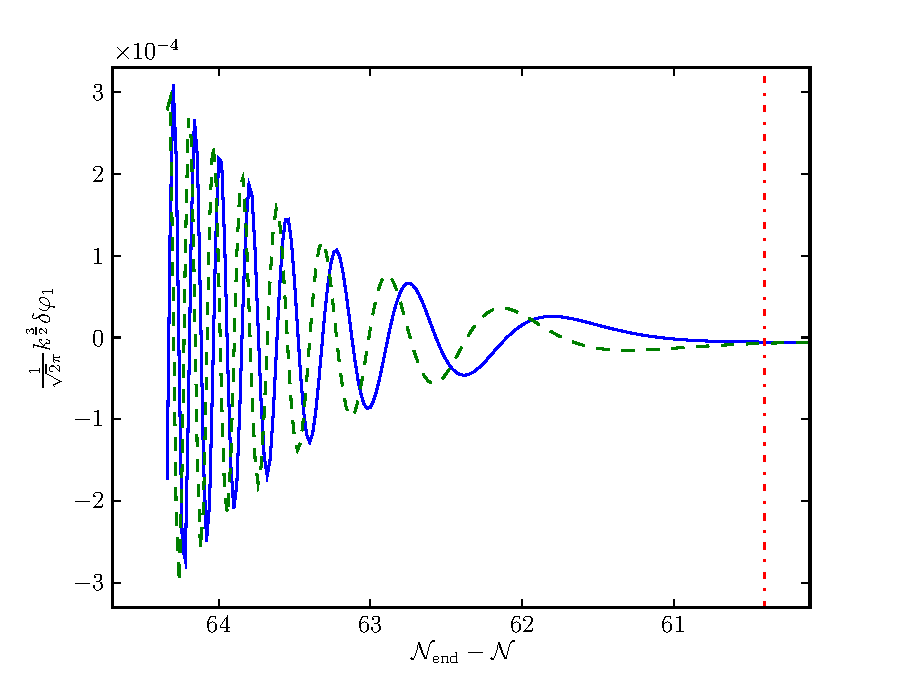
\includegraphics[width=0.8\textwidth]{numerical/graphs/dp1_kwmap}
 \caption[First Order Perturbation]{The first order perturbation $\dvp1$ rescaled by
$k^{3/2}/(\sqrt{2}\pi)$ from the beginning of the simulation until around
horizon crossing (red dot-dashed line). The real (blue) and imaginary (green
dashed) parts of the perturbation are shown for the scale $\kwmap$.}
\label{fig:dp1}
\end{figure}
% 

Figure~\ref{fig:dp2realimag} shows the evolution of the second
order perturbations for the scale $\kwmap$. As mentioned above, the
overall amplitude of the second order perturbation is many orders of
magnitude smaller than the corresponding first order one. In Figures~\ref{fig:dp1}
and \ref{fig:dp2realimag} the field values have been rescaled by
$k^{3/2}/(\sqrt{2}\pi)$ to allow for a better appreciation of the
magnitude of the resulting power spectra.
% 
\begin{figure}[htbp]
 \centering
 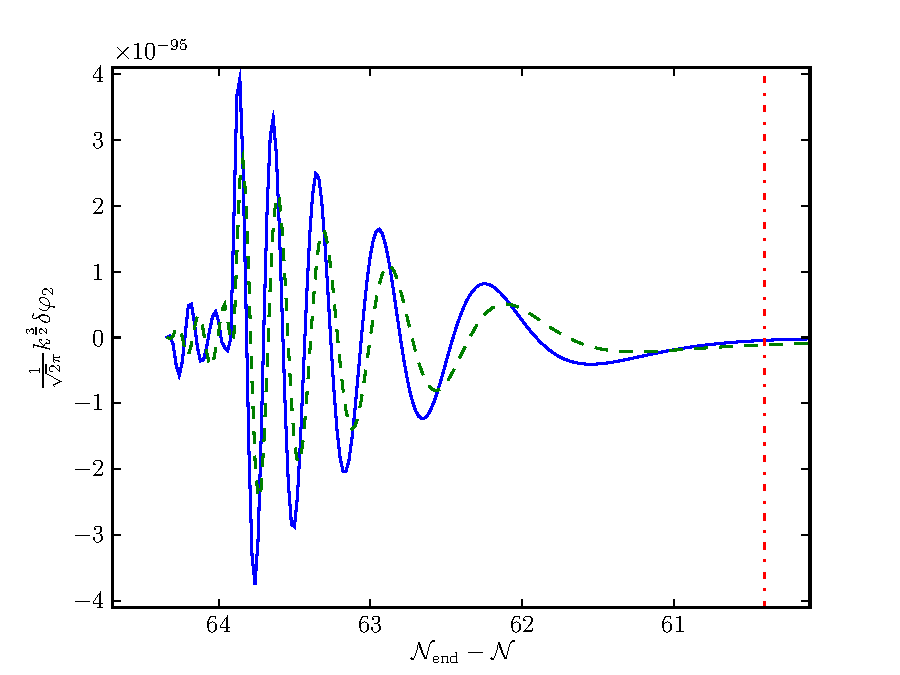
\includegraphics[width=0.8\textwidth]{numerical/graphs/dp2_kwmap}
 \caption[Second Order Perturbation]{The real (blue line) and imaginary (green
dashed) components of the
second order
perturbation $\dvp2(\kwmap)$ from the beginning of the simulation until around
the time
of horizon exit (red dot-dashed line).}
\label{fig:dp2realimag}
\end{figure}
% 
% % % % % % % % % % % % % % % % % % % % % % % % % % % % % % % % % % % 



The source term $S(\kvi)$ is calculated using \eq{eq:KG2-src-sr-aterms} at each time
step using the results of the first order and background simulations. This term
drives the production of second order perturbations as shown in
\eqs{eq:KG2-fourier-sr-num} and
\eqref{eq:KG2-fourier-sr-ntime}. Figure~\ref{fig:src-full} shows the
absolute magnitude of the source term for a single $k$ mode, $\kwmap$,
for all time steps calculated. 
The source term is large at early times, and closely follows the form
of the spectrum of the first order perturbations, as can be seen from
Figure~\ref{fig:Pphi-kwmap}.
% 
\begin{figure}[htbp]
\centering
\subfloat[Absolute magnitude of the source term.]{
 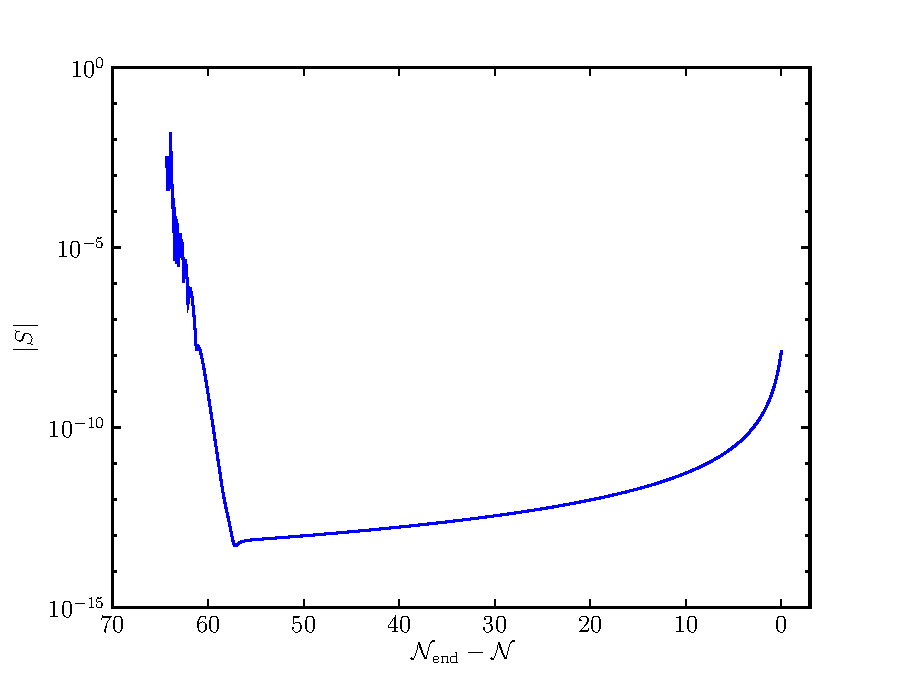
\includegraphics[width=0.8\textwidth]{numerical/graphs/src-kwmap-large}
\label{fig:src-full}
}\\
% 
\subfloat[First Order Power Spectrum of Scalar Perturbations][Power spectrum of
first order scalar
perturbations $\mathcal{P}^2_{\delta\varphi_1} =
\frac{k^3}{2\pi^2}|\delta\varphi_1|^2$.]{
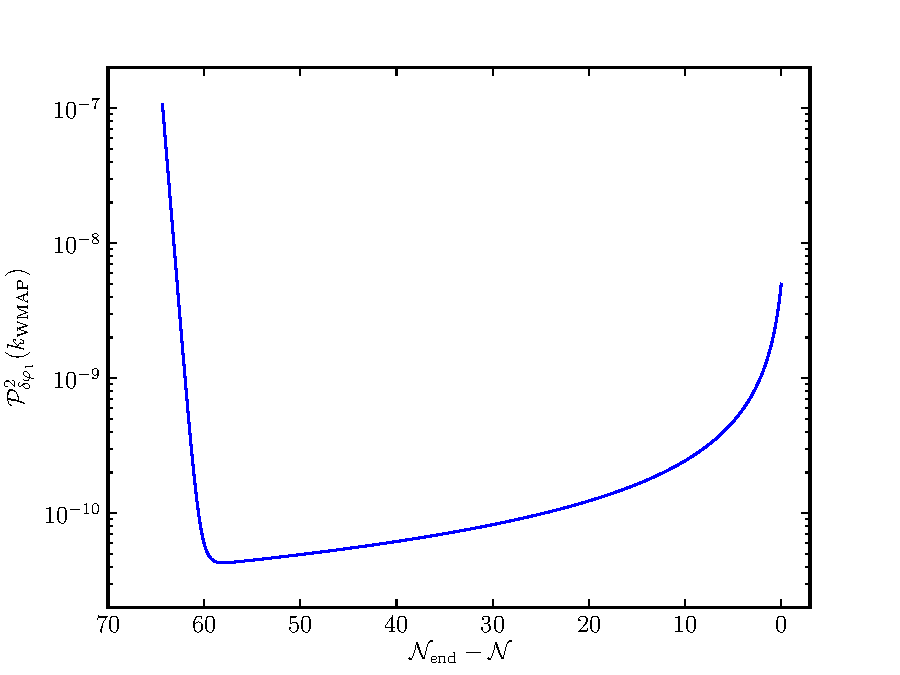
\includegraphics[width=0.8\textwidth]{numerical/graphs/Pphi-kwmap-nohoriz-large}
\label{fig:Pphi-kwmap}
}
\caption[Source Term and First Order Power Spectrum for $\kwmap$]{Source term and
first order power spectrum for the WMAP pivot scale $\kwmap$.}
\end{figure}
% 
Figure~\ref{fig:src-kwmap-3ranges} shows how the source term depends on
the choice of $k$ range.  After horizon crossing, the source term
is independent of the specific choice of $K_i$ ($i=1,2,3$). Before horizon crossing,
however, there is a
strict hierarchy with the smaller $k$ ranges, $K_1$ and $K_2$, leading to
smaller source
contributions.  As discussed in Section \ref{sec:tests-num}, $\Delta k$
should be at least as large as $\kmin$ in order for the error to be reduced to
a minimum. In Figure~\ref{fig:src-3ks} the source term is plotted at three different
values of $k$ for the range $K_1$. As $k$ increases, or equivalently the length scale
decreases, the magnitude of the source term after horizon crossing decreases. 
% 
\begin{figure}[htbp]
\centering
 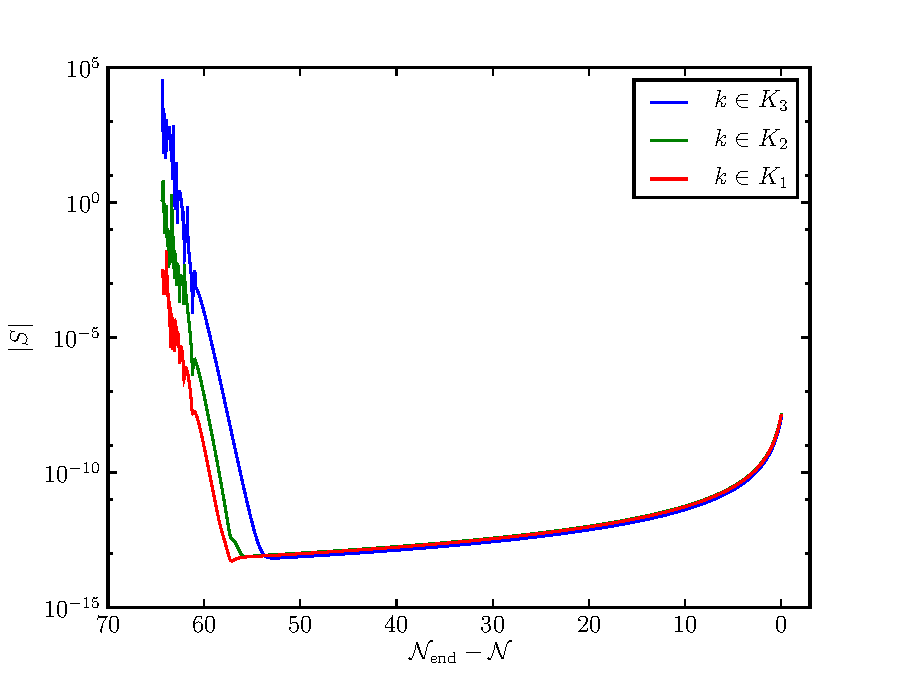
\includegraphics[width=0.8\textwidth]{numerical/graphs/src-kwmap-3ranges-large}
\caption[Comparison of Source Term for Different $k$ Ranges]{A comparison of the
source
term \eqref{eq:KG2-source-ntime}, for the scale $\kwmap=5.25\e{-60}\Mpl$, over the
three different ranges $K_1$,
$K_2$ and $K_3$, which were specified in \eq{eq:Kranges-res}. Before horizon
crossing there is a significant difference in the amplitude of the source term for
$\kwmap$. After horizon crossing, however, the magnitude of $S$ is independent of
the choice of $K_i$.
} 
\label{fig:src-kwmap-3ranges}
\end{figure}
% 
\begin{figure}[htbp]
\centering
 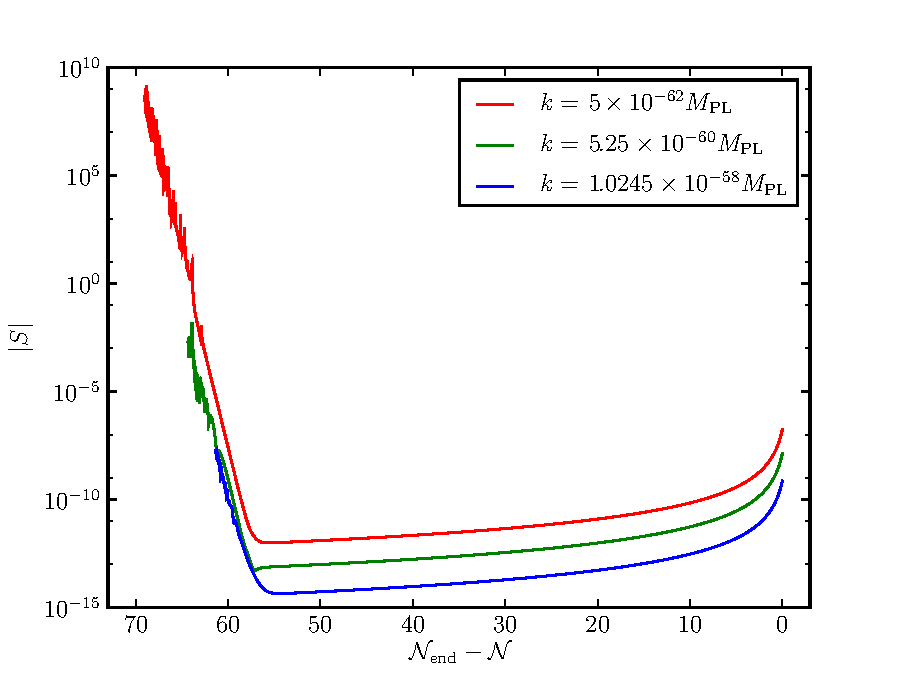
\includegraphics[width=0.8\textwidth]{numerical/graphs/src-3ks-large}
\caption[Source Term at Three Different Values of $k$]{The source term
\eqref{eq:KG2-source-ntime} for three different $k$
values in the $K_1$ range, including the WMAP
pivot scale, $\kwmap=5.25\e{-60}\Mpl$ (middle green line). As the value of $k$
increases or equivalently the scale decreases, the magnitude of the source term
decreases. The calculation of the source term for each $k$ value starts from the
time step at which the corresponding first order perturbation is initialised, \iec
when $k/aH = 50$.
}
\label{fig:src-3ks}
\end{figure}
% 
% 

%
It is informative to compare the magnitude of the source term with the
other terms in the second order evolution equation
(\ref{eq:KG2-fourier-sr-ntime}). We denote these other terms by $T$:
%
\begin{equation}
\label{eq:Tdefn}
 T(\kvi) = \left(3 + \frac{\dN{H}}{H}\right)
\dN{\dvp2}(\kvi)+ \left(\frac{k}{aH}\right)^2\dvp2(\kvi)
+\left(\frac{\Upp}{H^2}-{24 \pi G}(\dN{\vp_{0}})^2\right)
\dvp2(\kvi) \,.
\end{equation}
%
Figure~\ref{fig:src-vs-others} then shows the absolute magnitude of
both $S$ and $T$.  It is clear that for the scale $\kwmap$ the contributions to the
source term are only of comparable
magnitude during the early stages of the simulation.  
% 
Figure~\ref{fig:s-over-t-3ks}
shows a comparison of $|S|/|T|$ for three different $k$ values. 
The magnitude of $S$ is closer to that of the rest of the terms for the
larger $k$ mode.
A priori, the range of $k$ modes where $S$ will be large for a particular chosen
potential is not known. However, once the relevant values of $k$ have been
determined, it may be possible to significantly reduce the time
required for the simulation by restricting the calculation of $S$ to those regions
where it is important. Figure~\ref{fig:s-over-t-3ks} shows that it is not possible
to arbitrarily ignore the contribution of $S$ either inside or outside the horizon.
The full calculation on sub- and super-horizon scales is important for the evolution
of the second order perturbation at different scales.
%
\begin{figure}[htbp]
\centering
 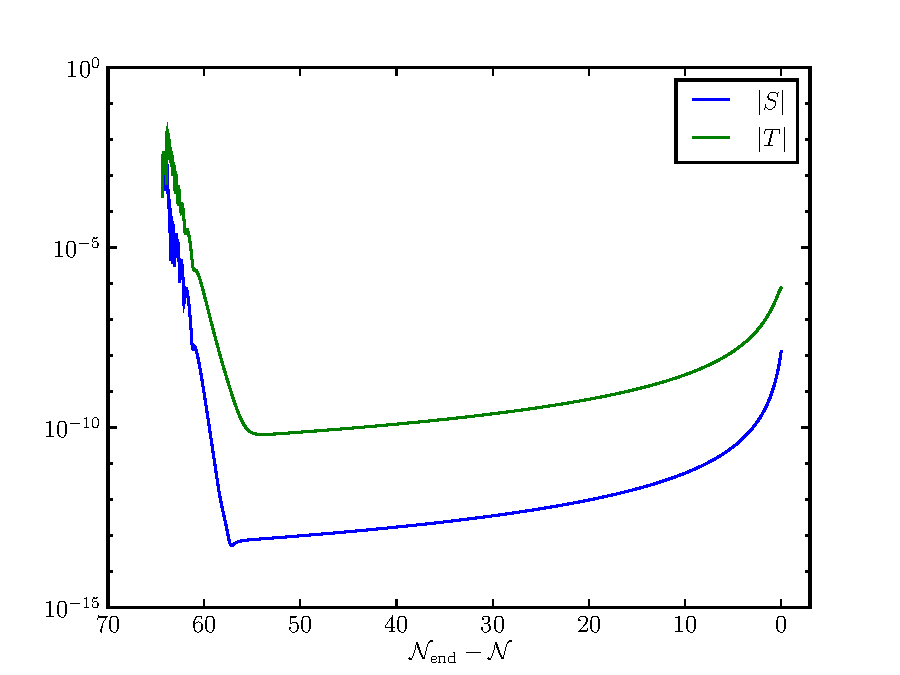
\includegraphics[width=0.8\textwidth]{numerical/graphs/src-vs-t-kwmap-large}
\caption[Source Term Compared to $T$ Term]{The source term (lower blue line), as
defined in \eq{eq:KG2-source-ntime}, is
compared with the $T$ term
(upper green line), as defined in \eq{eq:Tdefn}, for $\kwmap$. The source term is of
comparable magnitude at the beginning of the simulation.}
 \label{fig:src-vs-others}
\end{figure}
% 

\begin{figure}[htbp]
\centering
 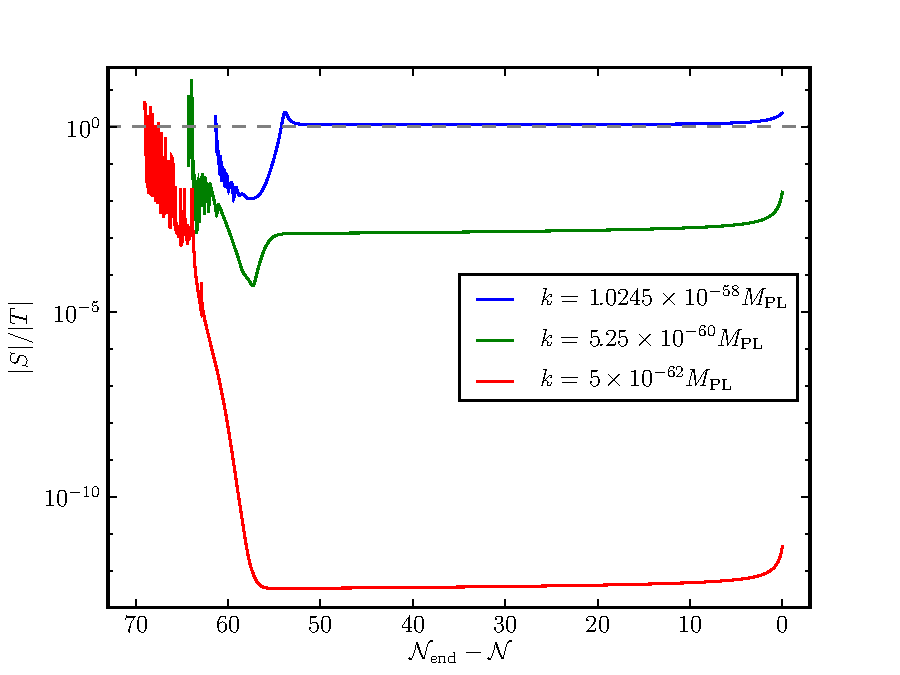
\includegraphics[width=0.8\textwidth]{numerical/graphs/s-over-t-3ks-large}
\caption[Quotient of $S$ and $T$]{The quotient of the $S$ term,
\eq{eq:KG2-source-ntime}, and the $T$ term, \eq{eq:Tdefn}, for three
different $k$ values in the range $K_1$,
including the WMAP pivot scale, $\kwmap=5.25\e{-60}\Mpl$.  
For small values of $k$ the source term is not comparable to the magnitude of $T$
after horizon crossing. However, for larger $k$ values (smaller scales) the two
terms have comparable magnitude.
It is, therefore,
important to calculate the source term over the full range of e-foldings.}
 \label{fig:s-over-t-3ks}
\end{figure}
% 
% 

% % % % % % % % % % % % % % % % % % % % % % % % % % % % % % % % % % %

In Figure~\ref{fig:src-kinit} the value of $|S|$ at the initialisation time
for each $k$ mode is shown. The initial magnitude of the source term is much
smaller for larger values of $k$ (smaller scales). 
Because the smaller $k$ modes begin their evolution earlier, the relative difference
in $|S|$ is not as pronounced when measured at a single time step (see for example
Figure~\ref{fig:src-3ks}).
It should also be remembered that the magnitude of the other terms in the second
order ODE is small for larger $k$ modes as shown by the ratio $|S|/|T|$ in
Figure~\ref{fig:s-over-t-3ks}.
% 
\begin{figure}[htbp]
\centering
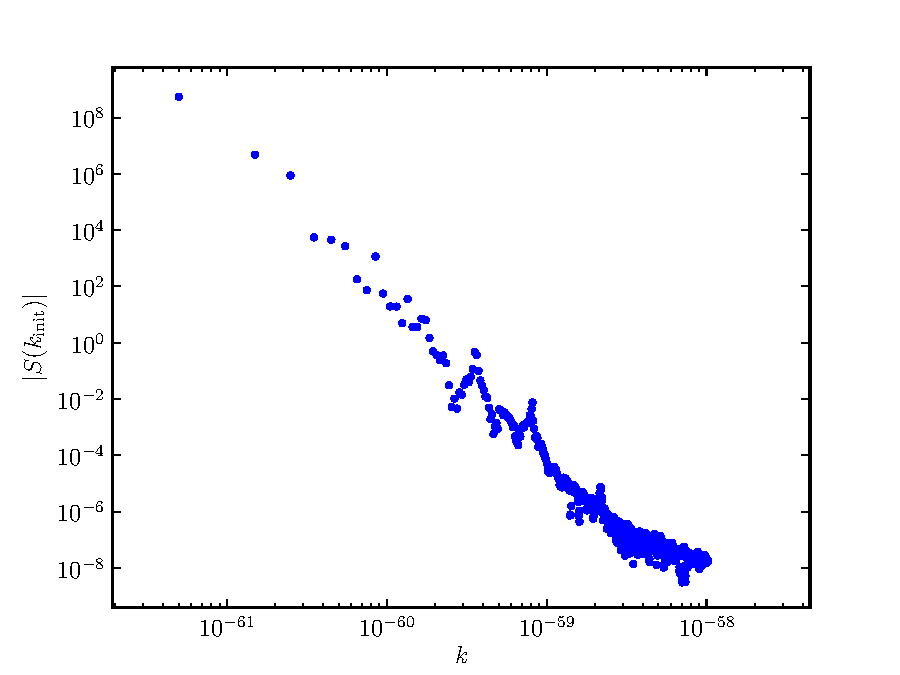
\includegraphics[width=0.8\textwidth]{numerical/graphs/src_kinit_log}
 \caption[Source Term at Initialisation]{The absolute magnitude of the source 
term at the initial start time for each $k$ value when $k/aH = 50$ deep inside
the
horizon. The results are for the range $K_1$.}
\label{fig:src-kinit}
\end{figure}
% 

The source term can also be compared at different time steps over all the $k$ values.
In Figure~\ref{fig:src-3ns} the upper blue line shows $|S(k)|$ around 69 e-foldings
before the end of
inflation when $\dvp1$ has been initialised for only the very smallest $k$
modes. The middle green
line shows $|S|$ when all $\dvp1$ modes have started to evolve. Finally, the lower
red line illustrates $|S|$
after all modes have exited the horizon, around 52 e-foldings before the end of
inflation.
% 
\begin{figure}[htbp]
\centering
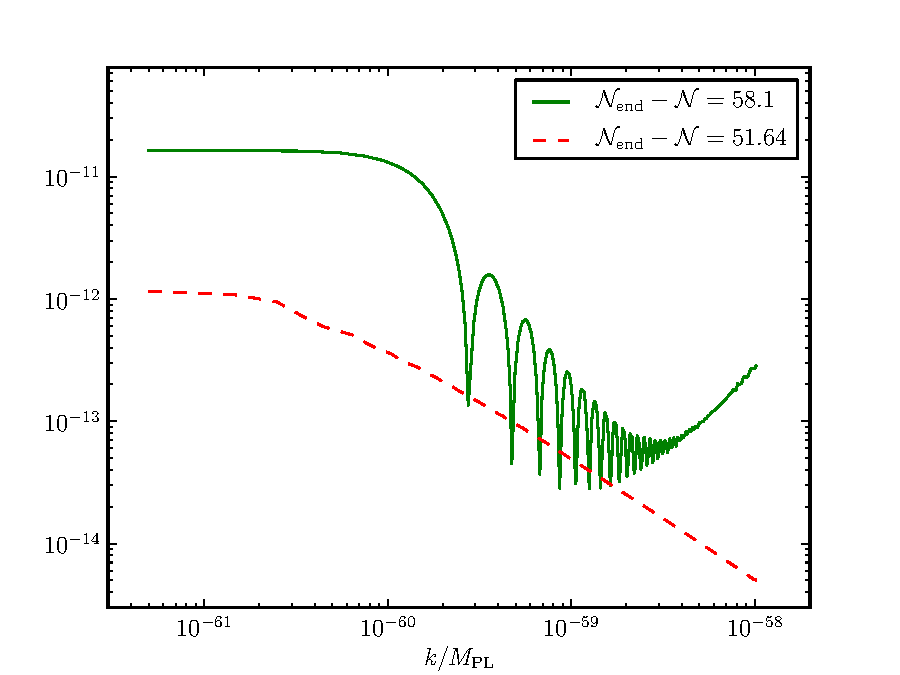
\includegraphics[width=0.8\textwidth]{numerical/graphs/src_3ns-large}
\caption[Source Term at Three Different Times]{The absolute magnitude of the source 
term for all $k$ values in the range $K_1$ at three different time steps. The upper
blue line shows $|S|$ at approximately $69$ e-foldings before the end of inflation
when
only the largest modes have been initialised. The middle green line shows $|S|$ when
all modes
have been initialised and the lower red dashed line when all modes have
exited the horizon.}
\label{fig:src-3ns}
\end{figure}
% 
% % % % % % % % % % % % % % % % % % % % % % % % % % % % % % % % 




% % % % % % % % % % % % % % % % % % % % % % % % % % % % % % % % 
% =========================================================== %
% % % % % % % % % % % % % % % % % % % % % % % % % % % % % % % %
\subsection{Comparison of Models}
\label{sec:compare-res}
% % % % % % % % % % % % % % % % % % % % % % % % % % % % % % % % 
% =========================================================== %
% % % % % % % % % % % % % % % % % % % % % % % % % % % % % % % %
All the results quoted so far have been for the quadratic potential. In this
section
the results for all four potentials will be compared using the $K_2$ range. 
% 
% 
\begin{figure}[htbp]
 \centering
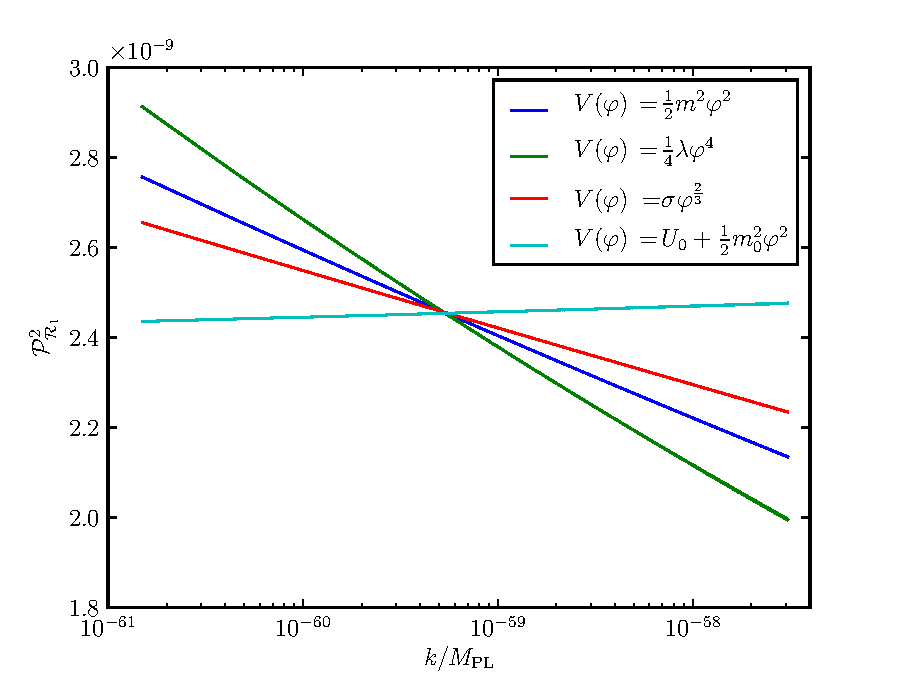
\includegraphics[width=0.8\textwidth]{numerical/graphs/cmp_Pr_allks-large}
\caption[Comparison of $\mathcal{P}^2_{\mathcal{R}_1}$ for the Four
Potentials]{Comparison of the power spectrum $\mathcal{P}^2_{\mathcal{R}_1}$ for
the four different models. The three models with potentials $\msqphisq$,
$\lambdaphifour$ and
$\phitwooverthree$ have red spectra ($n_s <1$) while the $\msqphisqwithV$
model has a blue spectrum ($n_s>1$).}
\label{fig:cmp-Pr}
\end{figure}
% 
Figure~\ref{fig:cmp-Pr} shows the power spectrum of first order curvature
perturbations, $\mathcal{P}^2_{\mathcal{R}_1}$, for each
potential. The $\msqphisq$, $\lambdaphifour$ and $\phitwooverthree$ models all
clearly have
a red spectrum with $n_s <1$. On the other hand, the $\msqphisqwithV$ model has
a blue
spectrum ($n_s>1$) when $U_0$ to chosen to be $5\e{-10}\Mpl^4$, as specified in
Section~\ref{sec:pots-num}. 
% 
The values of $n_s$ obtained for the four potentials are given in Table~\ref{table:ns-res}. 
% 
\begin{table}
\begin{center}
% use packages: array
\begin{tabular}{ccr}
\toprule
Potential & $n_s$ & $n_s - 1$ \\
\midrule
$\msqphisq$ & 0.965 & -0.035 \\ 
% \hline
$\lambdaphifour$ & 0.949 & -0.051 \\
% \hline 
$\phitwooverthree$ & 0.977 & -0.023 \\
% \hline 
$\msqphisqwithV$ & 1.002 & 0.002 \\
\bottomrule
\end{tabular}
\caption[Spectral Index Values for the Four Potentials]
{The spectral index for scalar perturbations for each of the four
potentials used. These values are calculated for the $\kwmap$ scale, five e-foldings
after it crosses the horizon. The potential parameters are listed in
Table~\ref{tab:params-num}. The value $U_0=5\e{-10}\Mpl^{4}$ was chosen to ensure
a blue spectrum ($n_s>1$).
}
\label{table:ns-res}
\end{center}
\end{table}


\begin{figure}[htbp]
\centering%
\subfloat[$V(\vp)=\msqphisq$]{
 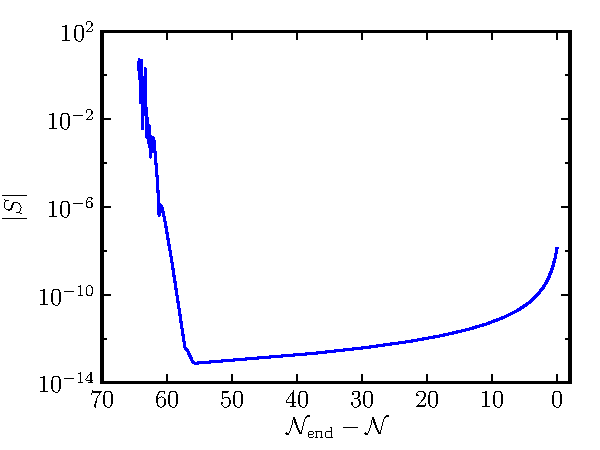
\includegraphics[width=0.43\textwidth]{numerical/graphs/src_onek_msqphisq-small}
}\qquad%
\subfloat[$V(\vp)=\lambdaphifour$]{
 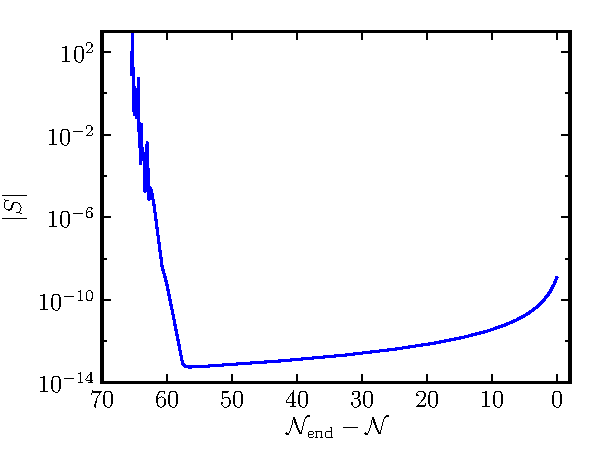
\includegraphics[width=0.43\textwidth]{numerical/graphs/src_onek_lambdaphi4-small}
}\\%
\subfloat[$V(\vp)=\phitwooverthree$]{
 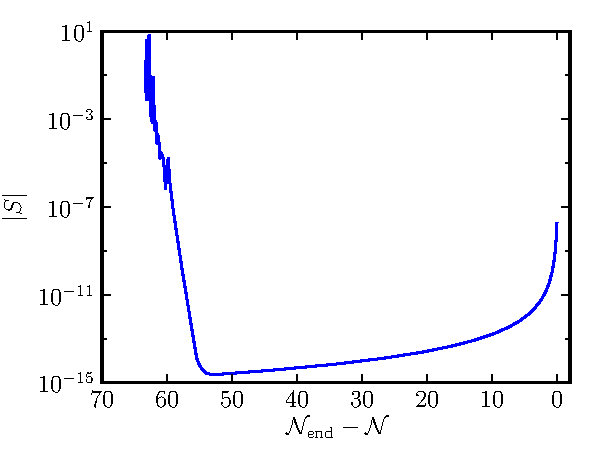
\includegraphics[width=0.43\textwidth]{numerical/graphs/src_onek_phi2over3-small}
}\qquad%
\subfloat[$V(\vp)=\msqphisqwithV$]{
 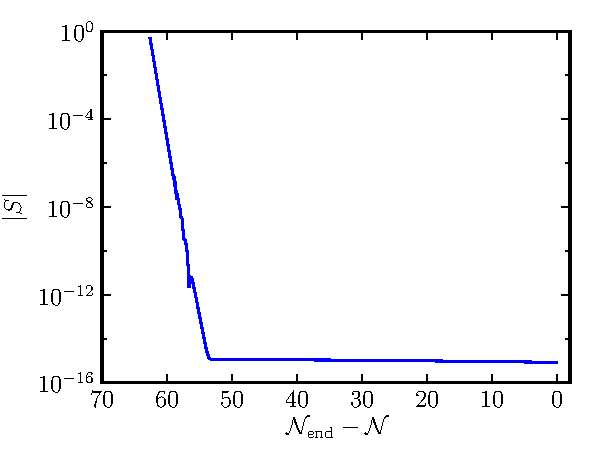
\includegraphics[width=0.43\textwidth]
  {numerical/graphs/src_onek_msqphisq_withV0-small}
}
\caption[Source Term for the Four Potentials]{Plots of the source
term for the
four different potentials studied.}
\label{fig:sourcecomparison-res}
\end{figure}
% 
The source term for each model is shown separately in Figure~\ref{fig:sourcecomparison-res} for
$\kwmap$ using the $K_2$ range\footnotemark. 
% 
\footnotetext{These plots use a different $k$ range to the ones comparing $V(\vp)=\msqphisq$ and
$\lambdaphifour$ in \Rref{hustonmalik}.}
% 
Although these terms are qualitatively similar,
differences between them are apparent. Figure~\ref{fig:cmp-src-kwmap} brings
together the source terms at $\kwmap$ to enable a direct comparison to be made. The
$\kwmap$ mode begins at different times for the
different models. Each result is therefore plotted in terms of the
initialisation time for that mode.  This change in duration is a consequence of
allowing $H$ to evolve during the calculation. 

\begin{figure}[htbp]
 \centering
 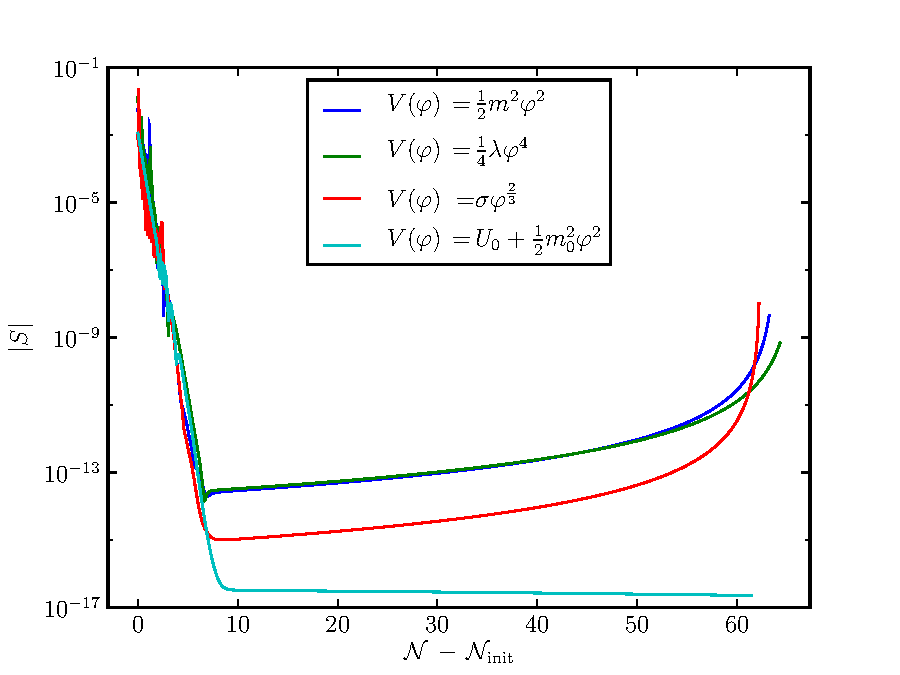
\includegraphics[width=0.8\textwidth]{numerical/graphs/cmp_src_kwmap-large}
 \caption[Comparison of Source Term for the Four Potentials]{Comparison of the
source term
evolution for the four different models. After horizon crossing the magnitude of the
source term is larger for the quadratic and quartic models than for the other two.
Towards the end of the numerical calculation there is a marked increase in $|S|$ for
three of the models as $\bar{\varepsilon}_H$ increases towards unity. The end time of
inflation is specified by hand for the contrived toy model, so this effect is
not seen.}
\label{fig:cmp-src-kwmap}
\end{figure}
% 

The source term results for the quadratic and quartic potentials are very similar.
Indeed, from horizon crossing to near the end of inflation the results appear to
coincide.
The $\lambdaphifour$ mode has a slightly longer duration and at late times is reduced in comparison
with the $\msqphisq$ one. Figure~\ref{fig:cmp-src-zoom-kwmap} shows that at early times the
relationship is more complicated with the $\lambdaphifour$ mode being larger for a significant
period.

In the early stages the amplitude of the $V(\vp)=\phitwooverthree$ model is very
similar to the other two
results described above. After horizon crossing, however, there is a significant drop
in the
amplitude of $S$ in comparison with the $\msqphisq$ and $\lambdaphifour$ models. This
continues
until late in the evolution when $|S|$ increases swiftly to reach levels above the
others.
The duration of the mode in this model is shorter than in the other two models
described so far. 

\begin{figure}[htbp]
 \centering
 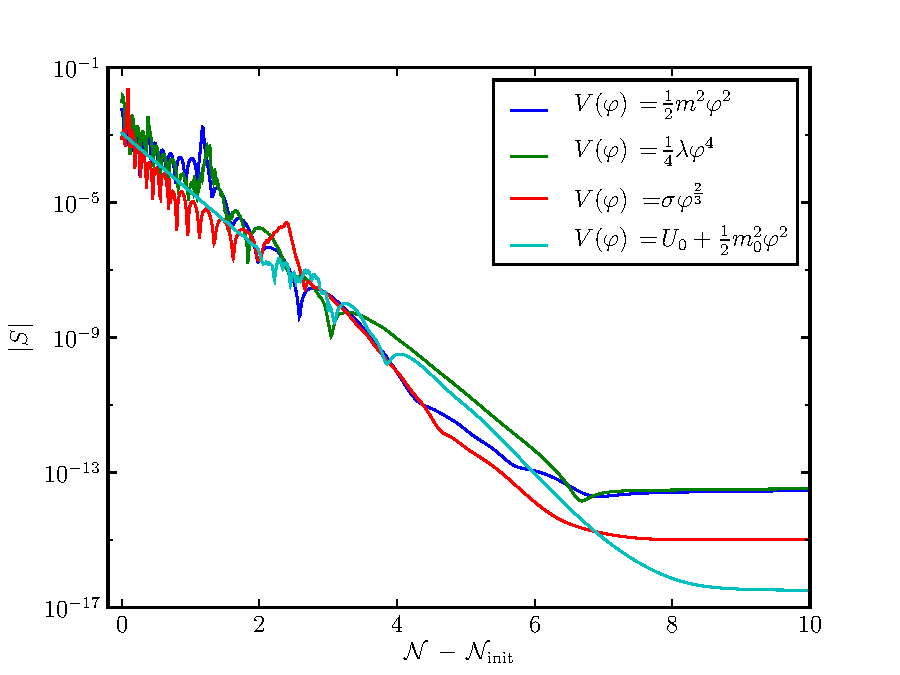
\includegraphics[width=0.8\textwidth]{numerical/graphs/cmp_src_kwmap_zoom-large}
 \caption[Comparison of Source Term at Early Times]{Comparison of the
source term evolution for the four different models at early times. This figure
highlights the early evolution of the four models shown in
Figure~\ref{fig:cmp-src-kwmap}. Before horizon crossing the magnitude of the source
term is comparable for each model. After horizon crossing differences between the
models become apparent.}
\label{fig:cmp-src-zoom-kwmap}
\end{figure}
% 

The fourth model, with potential $V(\vp)=\msqphisqwithV$, is a contrived toy model.
As described in Section~\ref{sec:pots-num}, in order to perform the single field
calculation, the end time of inflation must be specified by hand. In this simulation
$\vp\simeq 8$
is taken as the end time. The potential is extremely flat in this region and the
effect of this can
be seen in the source term of the model. Before horizon crossing it is of comparable magnitude to
the other terms. However, a steep decrease in $|S|$ ensures that it is a few orders
of magnitude
smaller than
the other terms after horizon crossing. In contrast to the behaviour of the other models, the source
term does not increase close to the end of inflation. This is due to the enforced end time cut-off
which means that $\bar{\varepsilon}_H$ does not become large.

In this section we have described the results for four different single field potentials. As
expected for single field slow roll models they exhibit similar properties. In the next section
plans to extend the calculation to deal with more interesting models will be outlined.

% % % % % % % % % % % % % % % % % % % % % % % % % % % % % % % % 
% =========================================================== %
% % % % % % % % % % % % % % % % % % % % % % % % % % % % % % % %
\section{Future Directions}
\label{sec:next-res}
% % % % % % % % % % % % % % % % % % % % % % % % % % % % % % % % 
% =========================================================== %
% % % % % % % % % % % % % % % % % % % % % % % % % % % % % % % %

There are many possible ways to improve the program outlined in
Chapter \ref{ch:numericalsystem}. Chief amongst these is the implementation of the
full second order source term given in \eqs{eq:SOKG-real-num} and
\eqref{eq:Fdvk1-fourier-num}. Although clearly
more complicated than the slow roll case of \eq{eq:KG2-fourier-sr-ntime},
only three more $\theta$ dependent terms need to be added to the $\A$--$\D$ terms
listed in \eq{eq:AtoD-num}.  The four potentials considered above all result in 
slow roll inflation. Therefore, it is not expected that
using the full source equation will result in an appreciably
different outcome in these models until near the end of the inflationary phase. Once
the field has stopped rolling slowly, new observable features are expected to
arise, as is indeed the case at first order. 


\eqs{eq:SOKG-real-num} and \eqref{eq:Fdvk1-fourier-num} must be written in
terms of $\N$, with the $\theta$ dependent terms grouped together, in order to set
up the numerical system completely at second order. 
The main equation
becomes
\begin{multline}
 \label{eq:fullso-res}
\ddN{\dvp2}(\kvi) + \left(3 + \frac{\dN{H}}{H}\right) \dN{\dvp2}(\kvi) +
\left(\frac{k}{aH}\right)^2 \dvp2(\kvi) \\
% 
+ \frac{1}{H^2}\left[ \Upp + 8\pi G\left(2\dN{\vp_0}\Uphi + 8\pi G
\left(\dN{\vp_0}\right)^2 \U \right)\right] \dvp2(\kvi)
% 
+ S_\mathrm{full}(\kvi) = 0\,,
\end{multline}
% 
where the full source equation is given by
% 
\begin{align}
\label{eq:fullsrc-res}
S_\mathrm{full}(\kvi) = \frac{1}{(2\pi)^2}\int \d q q^2 &\Bigg\{ 
% 
\frac{1}{\left(H\right)^2} \left[ \Uppp + 3(8\pi G)\dN{\vp_0}\Upp\right]
 \dvp1(\qvi) \A(\kvi, \qvi) \nonumber \\
% 
&+\frac{(8\pi G)^2 \dN{\vp_0}}{(aH)^2}\left[ 2a^2\dN{\vp_0}\Uphi +\dN{\vp_0}Q
-\frac{Q^2}{2(aH)^2}\right] \dvp1(\qvi) \A(\kvi, \qvi) \nonumber \\
% 
&- \frac{(8\pi G)^2}{(aH)^2}\frac{(\dN{\vp_0})^2 Q}{2} \dN{\dvp1}(\qvi)
\A(\kvi, \qvi) \nonumber \\
% 
&+ \frac{2(8\pi G)Q}{(aH)^2} \dvp1(\qvi)\wt{\C}(\kvi, \qvi) 
% 
+ \frac{8\pi G \dN{\vp_0}}{2} \dN{\dvp1}(\qvi) \wt{\C}(\kvi, \qvi) \Bigg\} \nonumber
\\
% 
&+ F_\mathrm{full}(\dvp1(\kvi), \dN{\dvp1}(\kvi))\,.
\end{align}
% 
The $F_\mathrm{full}$ term in \eq{eq:fullsrc-res} requires the use of three further
$\theta$
integrals in addition to those presented in \eq{eq:AtoD-num}. These take the form
% 
\begin{align}
\label{eq:efg-terms-res}
 \E(\kvi, \qvi) &= \int_0^\pi \cos^3(\theta) \sin(\theta) \dvp1(\kvi-\qvi)\d \theta
\,,\nonumber \\
% 
\F(\kvi, \qvi) &= \int_0^\pi \frac{\sin^3(\theta)}{|\kvi-\qvi|^2} \dvp1(\kvi-\qvi)\d
\theta \,,\nonumber \\
% 
\wt{\G}(\kvi, \qvi) &= \int_0^\pi \frac{\sin^3(\theta)}{|\kvi-\qvi|^2}
\dN{\dvp1}(\kvi-\qvi)\d \theta \,.
\end{align}
% 
It is worth noting that the term $\sin^3(\theta)/|\kvi-\qvi|^2$ tends to zero in the
limit where $k=q$ and
$\theta\rightarrow 0$.
% 
The $F_\mathrm{full}$ term can now be written in terms of $\E$, $\F$ and $\wt{\G}$:
\begin{align}
 \label{eq:fullfterm-res}
F_\mathrm{full} &= \frac{8\pi G}{(2\pi)^2}\frac{1}{(aH)^2} \int \d q\, q^2 \Bigg\{
\nonumber \\
% 
&  \dN{\vp_0}\Bigg[ \left(2k^2 + \left(\frac{7}{2} - \frac{8\pi
G}{4}(\dN{\vp_0})^2 \right)q^2 + \frac{3}{4}\frac{8\pi G}{(aH)^2} X^2 \right)
\dvp1(\qvi) \nonumber \\
% 
& \qquad + (8\pi G) Q \dN{\vp_0} \left(\frac{3}{4} + \frac{q^2}{k^2}\right)
 \dN{\dvp1}(\qvi) \Bigg] \A(\kvi, \qvi) \nonumber \\
% 
&+ \Bigg[ \left( 2Q \frac{q}{k} \left(1- \frac{8\pi G}{(aH)^2} Q \dN{\vp_0}\right)
-\frac{9}{2} \dN{\vp_0} k q - \dN{\vp_0} \frac{q^3}{k}\right) \dvp1(\qvi) \nonumber
\\
% 
&\qquad - 2Q (8\pi G) (\dN{\vp_0})^2\frac{q}{k} \dN{\dvp1}(\qvi)\Bigg] \B(\kvi, \qvi)
\nonumber \displaybreak[0]\\
% 
&+ \Bigg[ \left(-2 + (8\pi G)(\dN{\vp_0})^2 \left(\frac{1}{4} + \frac{1}{2aH}\right)
\right) Q \dvp1(\qvi) \nonumber \\
% 
&\qquad + \left(\frac{8\pi G}{4}(\dN{\vp_0})^2 -2\right) \dN{\vp_0} (aH)^2
\dN{\dvp1}(\qvi)\Bigg] \wt{\C}(\kvi, \qvi)\nonumber \\
% 
&+ \Bigg[ 2Q \frac{k}{q}\dvp1(\qvi) + \left(2\frac{k}{q}-\frac{q}{k}\right)
\dN{\vp_0} (aH)^2 \dN{\dvp1}(\qvi) \Bigg]\wt{\D}(\kvi, \qvi) \nonumber \\
% 
&+ (8\pi G) \dN{\vp_0} \Bigg[ \left(\frac{1}{4}(\dN{\vp_0})^2q^2 +
\frac{Q^2}{2(aH)^2}\right) \dvp1(\qvi) + \frac{Q}{2}\dN{\vp_0} \dN{\dvp1}(\qvi)
\Bigg] \E(\kvi, \qvi) \nonumber \displaybreak[0]\\
% 
&+ (8\pi G)^2 \dN{\vp_0} Q \Bigg[ -\frac{Q}{2(aH)^2}\left(\frac{k^2}{2}+q^2\right)
\dvp1(\qvi) - \frac{1}{4} \dN{\vp_0} k^2 \dN{\dvp1}(\qvi) \Bigg] \F(\kvi, \qvi)
\nonumber \\
% 
&+ (8\pi G)^2 (\dN{\vp_0})^2 \Bigg[ -\frac{Q}{2}\left(\frac{k^2}{2} +
\frac{q^2}{aH}\right)\dvp1(\qvi) -\frac{(aH)^2}{4}\dN{\vp_0}k^2 \dN{\dvp1}(\qvi)
\Bigg] \wt{\G}(\kvi, \qvi) \Bigg\} \,.
\end{align}
% 
\eqs{eq:fullsrc-res} and \eqref{eq:fullfterm-res} are clearly more complicated than
the slow roll versions used in
Chapter~\ref{ch:numericalsystem}. The numerical complexity is not significantly
greater, however, once the three terms in \eq{eq:efg-terms-res} have been calculated.
The running time of the full calculation will clearly be a significant constraint.

With this in mind, the performance of the numerical simulation could be improved by
analysing the most time consuming processes and investigating what
optimisations might be implemented. The current, perhaps
inelegant, procedure will allow any performance improvements to be benchmarked for
accuracy as well as for speed.
% 
As discussed above, $N_k$ was set to $1025$ for the test runs. This provides good
coverage of the
WMAP $k$ range, but it is not clear whether it sufficiently
approximates the integral to infinity for the source term.  Logistical factors,
including the running time and memory usage of the code,
restrict the choice of $N_k$. By optimising the routines
for reduced memory and increased speed it is hoped that the range of scales can be
extended and the resolution enhanced.


Beyond these considerations, the next significant step is to implement a multi-field
version of the system. This would allow the investigation of models that inherently
produce large second order perturbations. In \Rref{Malik:2006ir} the
second order Klein-Gordon equation for multiple fields was presented and upgrading
the
simulation to use these equations should be a straight-forward (if lengthy) process.
Extending the current data-structures and routines to a fixed number of extra fields
will increase the numerical complexity and the run-time of the code. 

For example, let us suppose that the second order perturbations of two scalar fields,
$\vp$ and $\chi$, are to
be calculated. Let $V$ denote the potential and $V_0$ its background value. As the
coding environment we have used can easily handle arrays of variables, it is useful
to write the equations in vector form. The following definitions will be used:
% 
\begin{align}
\label{eq:vector-defns-res}
 \bm{\vp_0} &= \begin{pmatrix}
                \vp_0 \\
		\chi_0
               \end{pmatrix} \,, &
% 
 &\bm{\dvp1} = \begin{pmatrix}
                \dvp1 \\
		\delta\chi_1
               \end{pmatrix} \,, &
% 
 &\bm{\dvp2} = \begin{pmatrix}
                \dvp2 \\
		\delta\chi_2
               \end{pmatrix} \,, \\
% 
 \bm{V_1} &= \begin{pmatrix}
             \Uphi \\
	     V_{,\chi} 
            \end{pmatrix} \,, &
% 
 &\bm{V_2} = \begin{pmatrix}
             \Upp & V_{,\vp\chi} \\
	     V_{,\chi\vp} & V_{,\chi\chi}
            \end{pmatrix} \,, &
% 
&\bm{V_3} = \begin{pmatrix}
            \Uppp & V_{,\vp\vp\chi} \\
	    V_{,\vp\vp\chi} & V_{,\vp\chi\chi} \\
	    V_{,\vp\chi\chi} & V_{,\chi\chi\chi}
           \end{pmatrix} \,.
\end{align}
% 
In conformal time the Friedmann equation becomes
% 
\begin{equation}
 \H^2 = \frac{8\pi G}{3} \left( \frac{1}{2}\left(\vp_0'\right)^2 
        + \frac{1}{2}\left(\chi_0'\right)^2 + a^2 \U \right) 
% 
= \frac{8\pi G}{3}\left( \frac{1}{2} \left( \bm{\vp_0}' \right)^{T} \bm{\vp_0}' + a^2 \U \right) \,,
\end{equation}
% 
where $\bm{\vp}^{T}$ denotes the transpose of $\bm{\vp}$.
% 
The background vector equation of motion is given by
% 
\begin{equation}
 \bm{\vp_0}'' + 2\H \bm{\vp_0}' + a^2 \bm{V_1} = \bm{0}\,,
\end{equation}
% 
where $\bm{0}$ is the zero vector.
The first order vector equation takes the form
% 
\begin{multline}
 \bm{\dvp1}''(\kvi) + 2\H \bm{\dvp1}'(\kvi) \\
 + \left( k^2 \bm{1}  + \bm{V_2} 
 + \frac{8\pi G}{\H}\left\{ 
  \bm{\vp_0}' \bm{V_1}^{T} + \bm{V_1}\left(\bm{\vp_0}'\right)^T
  + \frac{8\pi G}{\H}\U \bm{\vp_0}' \left(\bm{\vp_0}'\right)^T
\right\}
\right)\bm{\dvp1}(\kvi) = \bm{0}\,,
\end{multline}
% 
where $\bm{1}$ is the identity matrix.

We will outline the second order vector equation using the slow roll approximation.
In the multi-field case there are many more slow roll parameters than in the
single field scenario. Extending the definition of $\bar{\varepsilon}_H$ in
\eq{eq:bareps-defn-perts} to two fields gives
% 
\begin{align}
 \bar{\varepsilon}_\vp &= \sqrt{4\pi G} \left( \frac{\vp_0'}{\H} \right) \,,\\
 \bar{\varepsilon}_\chi &= \sqrt{4\pi G} \left( \frac{\chi_0'}{\H} \right)\,.
\end{align}
% 
There are now four $\eta_H$-type parameters corresponding to the different
combinations of second derivatives of $V$. These can be written together in matrix form
as
% 
\begin{equation}
 (\eta_{IJ}) = \bm{\eta}_H = \frac{a^2}{3\H^2} \bm{V_2} \,,
\end{equation}
% 
where $I,J = \vp,\chi$.
The magnitude of $\eta_{IJ}$ is only small in the adiabatic direction, so terms
including $\eta_{IJ}$ are included when making the slow roll approximation
\cite{Malik:2006ir}.

The second order, slow roll, vector equation for the perturbations is given by 
% 
\begin{align}
 \bm{\dvp2}''(\kvi) &+ 2\H\bm{\dvp2}'(\kvi) 
 + \left( k^2\bm{1} + a^2\bm{V_2} - 24\pi G \bm{\vp_0}' \left(\bm{\vp_0}'\right)^T \right)
       \bm{\dvp2}(\kvi) \nonumber\\ 
 &+ \bm{S}(\kvi) = \bm{0}\,,
\end{align}
% 
where the slow roll source term equation is
% 
\begin{align}
\label{eq:src-vector-res}
\bm{S}(\kvi) =\,  
&\frac{1}{(2\pi)^3}\int \d^3p\ \d^3q\ \delta^3(\kvi-\pvi-\qvi) \Bigg\{ \\
% 
&a^2 \Bigg[ 
\begin{pmatrix}
\dvp1(\pvi) & \delta \chi_1(\pvi) & 0  \nonumber\\
0           & \dvp1(\pvi)         & \delta \chi_1(\pvi) 
\end{pmatrix}
\bm{V_3}\bm{\dvp1}(\qvi) \nonumber \\
% 
&+ \frac{8\pi G}{\H}\left( 
    \bm{\dvp1}^T(\pvi) \bm{V_2} \bm{\dvp1}(\qvi)
\right) \bm{\vp_0}' \Bigg] \nonumber\\
% 
&+ \frac{16\pi G a^2}{\H}\left(\left(\bm{\vp_0}'\right)^T \bm{\dvp1}(\pvi) \right)
    \bm{V_2} \bm{\dvp1}(\qvi) \nonumber \\
% 
&+ \frac{8\pi G}{\H} \Bigg[ 2\frac{p_l q^l}{q^2} 
      \left( \left(\bm{\vp_0}'\right)^T \bm{\dvp1}'(\qvi) \right) \bm{\dvp1}'(\pvi)
 + 2p^2 \left( \left(\bm{\vp_0}'\right)^T \bm{\dvp1}(\qvi) \right) \bm{\dvp1}(\pvi) \nonumber \\
% 
&+\left( \frac{p_l q^l + p^2}{k^2}q^2 - \frac{p_l q^l}{2} \right) 
      \left( \bm{\dvp1}^T(\pvi) \bm{\dvp1}(\qvi) \right) \bm{\vp_0}' \nonumber \\
% 
&+\left(\frac{1}{2} -\frac{p_l q^l + q^2}{k^2}\right) 
      \left( \left(\bm{\dvp1}'\right)^T(\pvi) \bm{\dvp1}'(\qvi) \right) \bm{\vp_0}' \Bigg] \Bigg\}
\,.
\end{align}

Following the method of Section~\ref{sec:eqs-num}, the $\d^3p$ integral is evaluated
and the $\d^3 q$ integral is written in spherical polar coordinates. The $\theta$
dependent terms, which are equivalent to \eq{eq:AtoD-num} in the single field case,
are given by
% 
\begin{align}
\label{eq:AtoD-vectors-res}
 \A_\vp(\kvi,\qvi) &= \int_0^\pi \sin(\theta) \dvp1(\kvi-\qvi) \d\theta \,,
\nonumber \\ \displaybreak[0]
 \A_\chi(\kvi,\qvi) &= \int_0^\pi \sin(\theta) \delta \chi_1(\kvi-\qvi) \d\theta \,,
\nonumber\\ \displaybreak[0]
 \bm{\A}(\kvi,\qvi) &= \int_0^\pi \sin(\theta) \bm{\dvp1}(\kvi-\qvi) \d\theta \,,
\nonumber\\ \displaybreak[0]
 \bm{\B}(\kvi,\qvi) &= \int_0^\pi \cos(\theta)\sin(\theta) \bm{\dvp1}(\kvi-\qvi)
\d\theta \,,\nonumber\\ \displaybreak[0]
 \bm{\C}(\kvi,\qvi) &= \int_0^\pi \sin(\theta) \bm{\dvp1}'(\kvi-\qvi) \d\theta \,,
\nonumber\\
 \bm{\D}(\kvi,\qvi) &= \int_0^\pi \cos(\theta) \sin(\theta) \bm{\dvp1}'(\kvi-\qvi)
\d\theta \,.
\end{align}
% 
The first two equations are not vector equations but are needed for the explicit
matrix term in \eq{eq:src-vector-res}. We rewrite that equation with these
definitions to obtain:
% 
\begin{align}
 \bm{S}(\kvi) =\, &\frac{1}{(2\pi)^2}\int\d q \Bigg\{ \nonumber \\
% 
&a^2 q^2\Biggl[ \begin{pmatrix}
                 \A_\vp(\kvi,\qvi) & \A_\chi(\kvi,\qvi) & 0 \\
		 0                 & \A_\vp(\kvi, \qvi) & \A_\chi(\kvi, \qvi)
                \end{pmatrix}
		\bm{V_3} \bm{\dvp1}(\qvi) \nonumber \\
& \qquad +\frac{8\pi G}{\H} \left( \bm{\A}^T(\kvi,\qvi) \bm{V_2}
\bm{\dvp1}(\qvi)\right) \bm{\vp_0}'
	\Biggr] \nonumber \\
% 
&+ \frac{16\pi G}{\H}a^2 q^2 \left( \left(\bm{\vp_0}'\right)^T \bm{\A}(\kvi,\qvi) \right)
	\bm{V_2}\bm{\dvp1}(\qvi) \nonumber \\
% 
&+ \frac{8\pi G}{\H} \Bigg[ 2\left( \left(\bm{\vp_0}'\right)^T \bm{\dvp1}'(\qvi) \right)
	\left( kq \bm{\D}(\kvi,\qvi) - q^2 \bm{\C}(\kvi, \qvi) \right) \nonumber \\
% 
&\qquad +2q^2 \left( \left(\bm{\vp_0}'\right)^T \bm{\dvp1}(\qvi) \right)
	\left( (k^2 + q^2)\bm{\A}(\kvi,\qvi) - 2kq\bm{\B}(\kvi, \qvi) \right)\notag\\
% 
&\qquad + \left(\left[ \frac{3}{2}q^4 \bm{\A}^T(\kvi,\qvi) 
	- \left( \frac{1}{2}kq^3 + \frac{q^5}{k}\right) \bm{\B}^T(\kvi,\qvi)
	\right] \bm{\dvp1}(\qvi) \right) \bm{\vp_0}' \nonumber \\
% 
&\qquad + \left(\left[ \frac{1}{2}q^2 \bm{\C}^T(\kvi,\qvi) 
	- \frac{q^3}{k} \bm{\D}^T(\kvi,\qvi)
	\right] \bm{\dvp1}'(\qvi) \right) \bm{\vp_0}' \Bigg] \Bigg\} \,.
\end{align}
% 
This expression for $\bm{S}$ reduces to \eq{eq:KG2-src-sr-aterms} when only one
field is considered. At least in the slow roll case, the multi-field source term
equation is not considerably more complex than the single field one. The extra
numerical complexity arises from the calculation of the new $\theta$
dependent terms in \eq{eq:AtoD-vectors-res}. 




% 
% 
% 
% % % % % % % % % % % % % % % % % % % % % % % % % % % % % % % % 
% =========================================================== %
% % % % % % % % % % % % % % % % % % % % % % % % % % % % % % % %
\section{Discussion}
\label{sec:disc-num}
% % % % % % % % % % % % % % % % % % % % % % % % % % % % % % % % 
% =========================================================== %
% % % % % % % % % % % % % % % % % % % % % % % % % % % % % % % %

Part~\ref{part:numerical} of this thesis has described the numerical
solution of the evolution equations for second order scalar perturbations. The
closed form of the Klein-Gordon equation \eqref{eq:KG2-fourier-sr-num} has been
employed for the first time. We have shown that direct
calculation of the field perturbations beyond
first order using perturbation theory is readily achievable, although
it is non-trivial.

This first demonstration has been limited to considering
the slow roll approximation of the source term in \eq{eq:KG2-fourier-sr-num} which
is quadratic in first order perturbations. Slow roll has not been imposed on the
background or first order equations. Four different
potentials were
used to demonstrate the capabilities of the
system. The singularity at $k=0$, which arises as larger and larger
scales are considered, is avoided by implementing a cutoff at small
wavenumbers below $\kmin$. 
This is a pragmatic choice necessary for
the calculation.
It is also necessary to
specify a maximum value of $k$. This choice is dictated by computational
resources and with reference to observationally relevant scales. In
this demonstration, $k$ ranges have been used which are comparable with the
scales observed by the WMAP satellite. By comparing the analytical results of the
convolution integral with the numerical calculation, values of the parameters
$N_\theta, N_k$ and $\Delta k$ were chosen in such a way that the numerical error
was minimised. The convolution scheme that has been implemented
works best when $\Delta k>\kmin$.


We have seen explicitly that the second order calculations for the chosen
potentials can be completed once the cut-off for $\kmin$ is
imposed. As expected for these potentials the magnitude of second order perturbations
is extremely
suppressed in the slowly rolling regime, in comparison with the first order
amplitude.
We have also shown that the
evolution of the source term during the inflationary regime can be
readily calculated.


By computing the perturbations to second order, we have direct access
to the non-Gaussianity of $\dvp{}$. When used to investigate models
that predict a large non-linearity parameter, $\fnl$, this technique
could yield greater insight into the formation and development of the
non-Gaussian contributions by studying the effects of the different
terms in the source equation \eqref{eq:KG2-source-ntime}.
%
It was shown recently that $\fnl$ can be calculated directly from the field
equations \cite{Musso:2006pt,Seery:2008qj}, instead of
using the standard method based on a Lagrangian formalism
\cite{Maldacena:2002vr}. The method presented here
will
therefore eventually allow a full numerical calculation of $\fnl$ to be made.


In summary, we have demonstrated that numerically solving the closed
Klein-Gordon equation for second order perturbations is possible. The slow roll
version of the source term was used in the calculation, but
as described in Section~\ref{sec:next-res}, the extension of the system to include
the full source term is achievable. 
The analytic and numerical solutions for the convolution terms were
compared directly and found to be in good agreement.
The models used have been shown to have negligible second order
perturbations in line with known analytic results. 
